%----------------------------------------------------------------------------------------
% Regresión Logística
%----------------------------------------------------------------------------------------

Esta práctica introduce el concepto de \emph{regresión logística} para estimar probabilidades de datos, así como para la clasificación de estos. Se definirá el algoritmo de aprendizaje para la regresión logística y se verán sus similitudes con el Perceptrón.


\section{Objetivo}

Que el alumno conozca el concepto de \textit{regresión logística}, sus aplicaciones tanto para la estimación de distribuciones de probabilidad, como para clasificación. Que el alumno implemente el algoritmo de aprendizaje para poder estimar las probabilidades en un problema de clasificación binaria.

\begin{auxcode}
 \caption{Regresión logística}
 \centering
 \hurl{\auxprefix ia-regresion-logistica}
\end{auxcode}


\section{Introducción}

El aprendizaje supervisado comprende dos tipos de problemas básicos: 1) la clasificación; y 2) la regresión. Estos problemas pueden definirse a partir del tipo de valores que se esperan a la salida. En la clasificación, la salida de los métodos es una categoría, un valor discreto; por ejemplo $Y = \{0,1,2,...,N\}$. En el caso de la regresión, el valor de salida es continuo, ya sea $\mathbb{R}$ o un intervalo.

Los modelos de regresión lineal eligen una función lineal para estimar la dependencia entre las características $x$ de un ejemplar y la respuesta esperada $a(x)$. Una función lineal multivariable tendrá la forma: $$a(x) = \sum_{i=1}^n x_iw_i + \theta.$$
Los modelos lineales utilizan como base una función de este tipo para tratar los datos. Por ejemplo, el \textit{perceptrón} es un modelo lineal de clasificación, donde el valor final es determinado como 0, si $a(x)$ es un valor negativo, o 1 si es positivo.

Siguiendo estrictamenta las definiciones anteriores, en el caso de la regresión logística lineal, lo que buscamos no es una clasificación, sino una regresión. Concretamente, la regresión logística obtendrá una probabilidad; es decir, un valor continuo en el intervalo $[0,1]$.  Se trata de la composición de una \emph{función de distribución de probabilidad acumulada}\footnote{Formalmente la función de distribución acumulada para $X$ continua es $$F(x) = P[X \leq x] =\int_{-\infty}^{x} f(u) du$$ y la forma de la función $F(x)$ depende de la función de densidad de probabilidad $f(u)$.} actuando sobre la función lineal, para obtener un valor de regresión en el intervalo $[0,1]$. A continuación desarrollamos con más detalle el modelo de regresión logística.


\subsection{Regresión logística lineal}

Se trata de un modelo de regresión para obtener valores probabilísticos en una distribución binaria. Así, dado un dato de entrada $x$, representado como un vector, se obtiene la probabilidad de que este vector pertenezca a la clase 1 o a la clase 0. En particular, nos enfocaremos en la probabilidad de la clase 1.

Dado un conjunto de datos $X$ y el conjunto de clases $Y = \{0,1\}$, asumiremos que la distribución sobre $Y$ dado $X$ es binaria o Bernoulli, es decir, que si la probabilidad de $Y=1$ es $$p := P(Y=1|x)$$ entonces la probabilidad de la clase 0 se puede obtener de esta como $$P(Y=0|x) = 1-P(Y=1|x) = 1-p.$$


%La función logística, que es la función a partir de la cual podemos obtener $p$, se obtiene asumiendo que el logit de la distribución es lineal. El \emph{logit} es una estadística que determina el logaritmo de la cuota de la distribución.


La \emph{función logística} $\sigma(z)$ es una distribución de probabilidad acumulada simétrica que se puede elegir para mapear una predicción lineal al intervalo $[0,1]$, de forma que se aproxima a $0$ y $1$ en sus extremos de forma suave, se comporta semejante a la recta para probabilidades entre $0.2$ y $0.8$ y es invertible \parencite{Fox2016}.  De este modo obtenemos el modelo de regresión logística lineal, que estima $p$ como:
\begin{align*}
 p &= \sigma \left(\sum_{i=1}^n x_i + \theta \right) = \frac{1}{1 + e^{-\big(\sum_{i=1}^n x_i + \theta\big)}}
\end{align*}

Bajo este modelo, la \emph{función cuantil} de la función de distribución\footnote{``El \textit{cuantil} de orden $p$ es el valor de la variable $x_p$ que marca un corte de modo que una proporción $p$ de valores de la población es menor o igual que $x_{p}$''.  La función cuantil marca el punto de corte $x_p$ y es la inversa de la distribución de probabilidad acumulada. \hurl{https://es.wikipedia.org/wiki/Cuantil}} es lineal:
\begin{align}
 \sigma^{-1}(p) &= \sum_{i=1}^n x_i + \theta \label{eq:cuantil}
\end{align}

Al proceder a calcular explícitamente la inversa de $\sigma$ a partir de \eref{eq:cuantil} notamos lo siguiente:
\begin{align*}
 \frac{p}{1-p} &= e^{\sum_{i=1}^n x_i + \theta}
\end{align*}
donde el término de la izquierda es llamado la \emph{cuota} a favor de $Y=1$, pues entre mayor sea su valor, mayor es la probabilidad de que ocurra $Y=1$.\footnote{La cuota es una medida de la \emph{verosimilitud} de un evento, es decir, la probabilidad de haber observado un valor de una variable aleatoria, dados los parámetros de la función de densidad de probabilidad de la cual se obtuvo la muestra. \hurl{https://en.wikipedia.org/wiki/Likelihood_function}}  Al sacar el logaritmo de ambos lados obtenemos el \emph{logit}, el logaritmo de la cuota, y es éste el que estamos modelando con una función lineal:
\begin{align*}
logit := \ln \frac{p}{1-p} = \sum_{i=1}^n x_i + \theta
\end{align*}

El logit es igual a 0 cuando $ p = 1-p$, es decir, cuando el evento es aleatorio ($p = 0.5$), toma valores positivos cuando $p > 1-p$ y valores negativos cuando $p < 1-p$.

La función logística toma valores entre 0 y 1, y toma el valor $0.5$ cuando $$\sum_{i=1}^n x_i + \theta = 0$$ En la \fref{Fig:Logistic} se observa como los valores de 0 y 1 sólo se alcanzan en el límite. Los valores $w_i$ con $i=1,...,n$ y $\theta$ son los parámetros que se deben aprender. La función logística es entonces la función que determina el modelo de regresión logística.


\begin{figure}
 \centering
 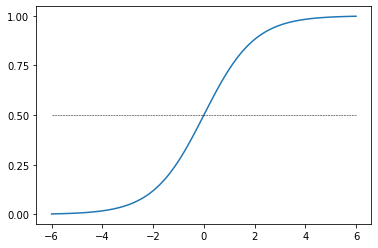
\includegraphics[scale=0.5]{regresion/logisticFunction}
 \caption{Función logística}\label{Fig:Logistic}
\end{figure}




\begin{definition}[Regresión logística]
La regresión logística es un modelo gráfico lineal para estimar probabilidades en distribuciones binarias. En este modelo, la distribución probabilística está definida por la función logística:
\begin{align*}
 \sigma(x; w, \theta) = \frac{1}{1 + e^{-\big(\sum_{i=1}^n w_i x_i + \theta\big)}}
\end{align*}
donde $w = \begin{pmatrix} w_1 & w_2 & \cdots & w_n \end{pmatrix}$ y $\theta$ son los parámetros del modelo que debemos aprender.
\end{definition}

El modelo gráfico que define la regresión logística se puede ver en la Figura~\ref{Fig:LinearReg}. Como se puede observar, la gráfica del modelo es similar a la de un modelo de Bayes Ingenuo; sin embargo, ambos modelos operan de forma diferente. Se dice que el modelo de Bayes Ingenuo es un modelo generativo, pues es capaz de generar nuevos ejemplares a partir de los patrones que aprende de los datos de entrenamiento; mientras que el modelo de regresión logística es un modelo discriminativo, pues se limita a distinguir entre clases.

\begin{figure}
 \centering
 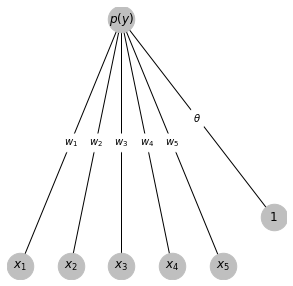
\includegraphics[scale=0.6]{regresion/RegressionModel.png}
 \caption{Modelo gráfico del modelo de regresión lineal}\label{Fig:LinearReg}
\end{figure}    




\subsection{Estimación del modelo}

Para aprender los parámetros de la regresión logística, utilizaremos el algoritmo de descenso por el gradiente. Básicamente, el algoritmo de descenso por el gradiente busca encontrar el mínimo de una función objetivo a partir de observar el comportamiento del vector gradiente. Este algoritmo usa como base el paso:

$$ x \leftarrow x - \alpha \nabla_x f(x) $$

que se repite iterativamente.  Es decir, en cada paso, actualizamos los valores de los parámetros restando el gradiente ponderado por un valor real $\alpha$. Al valor $\alpha$ se le conoce como taza de aprendizaje y funciona de manera idéntica que en el Perceptrón.  Para elegir un valor adecuado de $\alpha$ se usa como guía el comportamiento siguiente: si tras actualizar los paramétros el valor de la función objetivo se incrementa, nos indica que nos alejamos del mínimo, por lo que debemos reducir el valor de $\alpha$; por el contrario, si el valor disminuye, seguimos avanzando por esta dirección con esta taza para alcanzar el mínimo.

En el caso de la regresión logística, la función objetivo (ya que trabajamos con probabilidades) será la estimación por máxima verosimilitud logarítmica. Pero esta función busca maximizar los valores por lo que tomaremos el negativo de esta función.\footnote{A la función objetivo definida de esta forma también se le conoce como entropía cruzada.} Esta función está dada como:

\begin{equation*}
    J(w, \theta) = - y \ln\big( \sigma(x; w, \theta)\big) - (1- y) \ln\big( 1-\sigma(x; w, \theta) \big)
\end{equation*}

Dado que tenemos una distribución binaria, se toman dos términos: el término $y \ln\big( \sigma(x; w, \theta)\big)$ que corresponde a la probabilidad de la clase 1, y el término $(1-y) \ln\big( 1-\sigma(x; w, \theta)\big)$ que corresponde a la probabilidad de la clase 0. Claramente si el dato $x$ de entrada pertenece a la clase 1, minimizar el primer término corresponde a maximizar la probabilidad $\sigma(x; w, \theta)$. Análogamente, se maximiza la probabilidad de la clase 0 cuando los datos de entrada son de esta clase.

Para aplicar el descenso por el gradiente debemos obtener el vector gradiente, lo que implica obtener las derivadas parciales de la función objetivo con respecto a los parámetros entrenables. Podemos observar que:

\begin{align*}
    \frac{\partial J }{\partial w_i} &= - y \frac{\partial}{\partial w_i} \ln\big( \sigma(x; w, \theta)\big) - (1- y) \frac{\partial }{\partial w_i}  \ln\big( 1-\sigma(x; w, \theta) \big) \\
        &= \big( \sigma(x; w, \theta) - y \big) x_i 
\end{align*}

Pues la derivada de la sigmoide es $\sigma(x; w, \theta)\big(1-(x; w, \theta)\big)$ y desarrollando por los dos casos, $y=1$ y $y=0$, podemos obtener el resultado. De igual forma es fácil notar que para $\theta$ tenemos:

\begin{align*}
    \frac{\partial J }{\partial \theta} &= - y \frac{\partial}{\partial \theta} \ln\big( \sigma(x; w, \theta)\big) - (1- y) \frac{\partial }{\partial \theta}  \ln\big( 1-\sigma(x; w, \theta) \big) \\
        &= \big( \sigma(x; w, \theta) - y \big)
\end{align*}

En el \pref{alg:AlgReg} se describe la implementación del aprendizaje en la regresión logística.


\begin{algorithm}
 \caption{Algoritmo de aprendizaje para la regresión logística}\label{alg:AlgReg}
 \begin{algorithmic}
  \Function{Ajusta-Regresión-Logística-Lineal}{$X$, $Y$, $\alpha$, $T$}
    \State $w, \theta \leftarrow$ \textsc{Random}$(w, \theta)$
    \For{$t \leftarrow 1$ hasta $T$}
        \For{ $x, y \in X,Y$ }
            \State $f(x) \leftarrow \sigma(x; w, \theta) $
            \State $w \leftarrow w - \alpha \big( f(x) - y \big) x $
            \State $\theta \leftarrow \theta - \alpha \big( f(x) - y \big) $
        \EndFor
    \EndFor
    \State \textbf{return} La función $\sigma(\cdot; w, \theta)$ con parámetros óptimos
  \EndFunction
 \end{algorithmic}
\end{algorithm}

El algoritmo para aprendizaje en regresión logística debe tomar un conjunto de datos de entrenamiento $X$ y las clases cuyas probabilidades se desean estimar $Y$. Además se indica la taza de aprendizaje $\alpha$ y el número máximo de iteraciones $T$. Los valores de $w$ y $\theta$ se inician aleatoriamente y se ajustan hasta obtener una solución adecuada.


\subsection{Clasificación con regresión logística}

El modelo de regresión logística permite obtener la probabilidad de una clase dado un vector de entrada. Con esta probabilidad se puede realizar una clasificación, pues sabemos que la probabilidad de la clase 1 está dada por la función logística, mientras que la probabilidad de la clase 0 se podrá obtener fácilmente de esta. Por tanto, podemos definir una función de clasificación a partir de la regresión logística como sigue:

\begin{equation*}
    \hat{y} = \begin{cases} 1 & \text{si } \sigma(x; w, \theta) \geq 0.5 \\
        0 & \text{si } \sigma(x; w, \theta) < 0.5 \\
    \end{cases}
\end{equation*}

Está función es similar a la función $\arg\max_y P(Y=y|x)$ pues toma como clase aquella cuya probabilidad sea la más alta, pues si la clase 0 es más alta, dado que $P(Y=0|x) = 1-\sigma(x; w, \theta)$, entonces necesariamente la clase 1 (cuya probabilidad es $P(Y=1|x) = \sigma(x; w, \theta)$ ) será más baja; y viceversa. También podemos notar que, como señalamos anteriormente $\sigma(x; w, \theta) = 0.5$ cuando $\sum_{i=1}^n w_i x_i + \theta = 0$ (véase Figura~\ref{Fig:Logistic}), la clasificación corresponde a la función escalón del Perceptrón; es decir, a la función dada por:

\begin{equation*}
    \hat{y} = \begin{cases} 1 & \text{si } \sum_{i=1}^n w_i x_i + \theta \geq 0 \\
        0 & \text{si } \sum_{i=1}^n w_i x_i + \theta < 0 \\
    \end{cases}
\end{equation*}

En conclusión, podemos ver que la regresión logística está ampliamente relacionada con el Perceptrón. En la Figura~\ref{Fig:LogistData} se puede ver un conjunto de datos para entrenar el modelo a la izquierda, y las regiones de clasificación que aprende el modelo a la derecha. Claramente, por lo que acabamos de señalar de su relación con el Perceptrón, la clasificación realizada por el modelo de regresión será lineal.

\begin{figure}
 \centering
 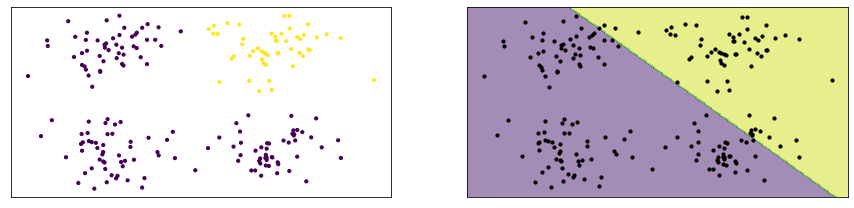
\includegraphics[width=1.0\textwidth]{regresion/LogisticData}
 \caption{A la izquierda los datos de entrenamiento, a la derecha las regiones de clasificación que se obtienen al entrenar el modelo.}\label{Fig:LogistData}
\end{figure}






\section{Desarrollo}

En esta práctica se implementará el modelo de regresión logística lineal y el algoritmo de aprendizaje para esta en un conjunto de datos lógico. Se propone generar un conjunto de datos en base al problema lógico \textsc{And}, pero introduciendo ruido para dispersar los datos en el espacio $\mathbb{R}^2$. Se entrenará un modelo de regresión logística y se obtendrán las probabilidades de que los datos pertenezcan a una clase o a otra.



\subsection{Implementación}

Para la implementación del código se manejarán arreglos en \code{numpy} y se definirá una clase para el modelo de regresión lineal. Esta clase deberá tener las funciones \code{fit}, \code{predict\_proba} y \code{predict}. Se deberán seguir los siguientes pasos:


\begin{itemize}
    \item Se generarán 200 ejemplos de entrenamiento definidos por la función \textsc{And} más un ruido. La función \textsc{And} está dada por la tabla de verdad:
    \begin{center}
        \begin{tabular}{ l l | c }
          $x_1$ & $x_2$ & $Salida$\\ \hline
          0 & 0  & 0 \\ \hline
          0 & 1 &  0  \\ \hline
          1 & 0 & 0  \\ \hline
          1 & 1 & 1  \\
        \end{tabular}
    \end{center}
    Se generarán 150 datos para la clase 0 y 50 datos para la clase 1. Para que estos datos sean variados, se les sumará ruido gaussiano. Se sugiere generar el ruido de la siguiente forma:
    \begin{center}
        \code{numpy.random.normal(loc=0,scale=1,size=(200,2))}
    \end{center}
    Esto generará ruido con media 0 y varianza 1 para los 200 datos de dos dimensiones. Se sumará a los datos este ruido escalado por un factor; se sugiere escalar el ruido por un factor entre 0.1 y 0.2.

    \item Se generará la clase \code{LogisticRegression}. Dentro de esta clase, se definirán las funciones \code{fit}, \code{predict\_proca} y \code{predict}.

    \item La función \code{predict\_proba} tomará como argumento un vector o varios vectores de entrada $x$ y devolverá la probabilidad de clase de estas entradas. Puede utilizarse esta función dentro de la función de entrenamiento \code{fit}.

    \item La función \code{fit} deberá tomar como argumentos los datos $X$ y sus clases $Y$ para el entrenamiento; además se deberá indicar la taza de aprendizaje (se sugiere un valor de 0.1) y un número máximo de iteraciones (se sugiere 100). Esta función ejecutará el algoritmo de aprendizaje (\pref{alg:AlgReg}). Se sugiere inicializar los parámetros de manera aleatoria con valores en el intervalo $[-0.5,0.5]$.

    \item La función \code{predict} tomará como argumento un vector o varios vectores de entrada $x$ y devolverá la clase propuesta para estas entradas. Es decir, esta función se encargará de clasificar los datos de entrada.

    \item Se sugiere comparar los resultados de clasificación con aquellos obtenidos con el Perceptrón. 
\end{itemize}


\subsection{Requisitos y resultados}

Se tendrá que entregar la clase \code{LogisticRegression} adecuadamente programada y documentada. Como se ha mencionado, la clase deberá contener las funciones \code{fit}, \code{predict\_proba} y \code{predict}, todas estas adecuadamente realizadas y funcionando de la manera indicada. Además, se usará esta clase para entrenar y obtener las clases de los datos que ya se han indicado.  Se otorgará un punto extra a quien incluya un reporte de su comparación con los resultados obtenidos con el perceptrón.
